\documentclass[14pt,aspectratio=169,dvipsnames,table]{beamer}
\usepackage{hastingstheme}
\titlegraphic{
\includegraphics[scale=.35]{static_figures/du_bn.pdf}}
\author{\large Massimiliano Fasi}
\date{}

\usepackage[T1]{fontenc}

\usepackage{amssymb}
\usepackage{tcolorbox}
\usepackage{hf-tikz}
\usepackage{listings}
\colorlet{lstbg}{Purple!0.4} % stack exchange shade
\lstset{%
  language=C,
  frame=single,
  backgroundcolor=\color{lstbg}
}

\usepackage[english]{babel}
\usepackage[utf8]{inputenc}
\usepackage[T1]{fontenc}
\usepackage{mathdots}
% \usepackage{stmaryrd}
\usepackage{mathtools}
\usepackage{verbatim}
\usepackage{mathtools}

% Algorithms
\usepackage[vlined,linesnumbered,algo2e]{algorithm2e}
\DontPrintSemicolon
\IncMargin{1em}
\SetInd{0.4em}{0.7em} % Reduce indentation (before/after vertical line)

\let\oldnl\nl
\newcommand{\nonl}{\renewcommand{\nl}{\let\nl\oldnl}} % Remove line number
\newcommand{\funcomment}[1]{\nonl$\triangleright$ \textit{#1}}
\SetKwComment{Comment}{$\triangleright$\ }{}
\makeatletter
\newcommand{\algorithmstyle}[1]{\renewcommand{\algocf@style}{#1}}
\makeatother

% Remove line number from selected lines
\newcommand{\pushline}{\Indp}% Indent
\newcommand{\popline}{\Indm\dosemic}% Undent
\let\oldnl\nl% Store \nl in \oldnl
\renewcommand{\thealgocf}{}
\renewcommand{\thefigure}{\!\!}

\usepackage{textpos}
\usepackage{appendixnumberbeamer}

% tabs
\usepackage{tabularx}
\usepackage{booktabs}
\usepackage{diagbox}
\usepackage{colortbl}
\usepackage{multirow}
\usepackage{setspace}
\usepackage{array}
\usepackage{hyperref}
\usepackage{varwidth}
\usepackage{xspace}
\usepackage{rotating}

% figs
\usepackage{graphics}
\usepackage{background}
\usepackage{tikz,pgfplots,ifthen}
\pgfplotsset{compat=1.16}
\usepackage{pgfplotstable}
\usetikzlibrary{intersections}
\usetikzlibrary{matrix}
\usetikzlibrary{fit}
\usetikzlibrary{backgrounds}
\usetikzlibrary{decorations.pathreplacing}
\usepgfplotslibrary{statistics}
\usepgfplotslibrary{fillbetween}
\usetikzlibrary{positioning}
\usetikzlibrary{external}
% \tikzset{external/force remake=false}
% \tikzexternalize[optimize=true,prefix=figs/]
% \tikzsetnextfilename{sisd}
\usetikzlibrary{calc}
% \input{tikz.tex}

\newcommand{\conj}[1]{\ensuremath{\overline{#1}}}

\newcommand{\divides}{\mid}
\newcommand{\notdivides}{\nmid}

\usepackage{style}

\makeatletter
\renewcommand*\env@matrix[1][\arraystretch]{%
  \edef\arraystretch{#1}%
  \hskip -\arraycolsep
  \let\@ifnextchar\new@ifnextchar
  \array{*\c@MaxMatrixCols c}}
\makeatother

% \definecolor{palette1}{RGB}{226, 149, 120}
% \definecolor{palette2}{RGB}{  0, 109, 119}
% \definecolor{palette3}{RGB}{131, 197, 190}
% \definecolor{palette4}{RGB}{237, 246, 249}
% \definecolor{palette5}{RGB}{255, 221, 210}

% \definecolor{palette1}{RGB}{255, 213, 58}
% \definecolor{palette2}{RGB}{104, 36, 109}
% \definecolor{palette3}{RGB}{203, 168, 177}
% \definecolor{palette4}{RGB}{182, 170, 167}
% \definecolor{palette5}{RGB}{218, 205, 162}
% \definecolor{palette6}{RGB}{190, 30, 45}


\colorlet{titlepagebgcolor}{palette2!80!Black}
% \colorlet{bgcolor}{palette4!100!black}
\colorlet{textcolor}{palette3!40!Black}

\setbeamercolor{block title}{fg=palette4!30!Black, bg=palette3!60!white}
\setbeamercolor{block body}{fg=textcolor,bg=palette3!40!white}

\setbeamercolor{title}{fg=palette5}
\setbeamercolor{author}{fg=palette4!20!white}

% \setbeamercolor{frametitle}{fg=palette1!100!white}

% \newcommand{\answer}[1]{{\vspace{3pt}\color{MidnightBlue}\textit{#1}}}
\newcommand{\myplus}{\textcolor{ForestGreen}{%
    \raisebox{2.5pt}{\rotatebox{90}{\bf\guilsinglright}}}}
\newcommand{\myminus}{\textcolor{Orange}{%
    \raisebox{2.5pt}{\rotatebox{90}{\bf\guilsinglleft}}}}
\newcommand{\mybad}{\textcolor{BrickRed}{%
    \raisebox{0.5pt}{\rotatebox{90}{\bf\guillemotleft}}}}

\newcommand{\codeslide}[2]{%
  \begin{frame}[fragile]
    \frametitle{Will the compiler vectorise this?}
\begin{lstlisting}
#1
\end{lstlisting}
  \end{frame}}

\begin{document}

\title{\firasemibold\color{White}%
  {\fontsize{20}{0}\selectfont SESSION 8\\
    \fontsize{34}{34}\selectfont Vectorisation \&\\data layout\par}}
\titleslide




\begin{frame}
  \frametitle{Scalar and vector operations}
  \begin{columns}
    \begin{column}{0.3\textwidth}
      \begin{equation*}
        \phantom{%
          \begin{bmatrix}
            z_0 \\ \vdots \\ z_n
          \end{bmatrix}}
        z \gets x + y
        \phantom{%
          \begin{bmatrix}
            z_0 \\ \vdots \\ z_n
          \end{bmatrix}}
      \end{equation*}\centering
      \structure{Scalar operation}
    \end{column}

    \begin{column}{0.3\textwidth}
      \begin{equation*}
        \begin{bmatrix}
          z_0 \\ \vdots \\ z_n
        \end{bmatrix}
        \gets
        \begin{bmatrix}
          x_0 \\ \vdots \\ x_n
        \end{bmatrix}
        +
        \begin{bmatrix}
          y_0 \\ \vdots \\ y_n
        \end{bmatrix}
      \end{equation*}\centering
      \structure{Vector operation}
    \end{column}
  \end{columns}

  \vskip 21pt

  \structure{Two realizations}\\[-10pt
  ]
  \begin{itemize}[itemsep=7pt]
  \item lockstepping (GPUs SIMT)
  \item large vector registers (x86 extensions)
  \end{itemize}
\end{frame}





\newcommand{\drawcube}[8]{%
  \draw[rounded corners=0.05pt,draw=#7,fill=#8] (#1,#2,#3) -- ++(-#4,0,0) -- ++(0,-#5,0) -- ++(#4,0,0) -- cycle;
  \draw[rounded corners=0.05pt,draw=#7,fill=#8] (#1,#2,#3) -- ++(0,0,-#6) -- ++(0,-#5,0) -- ++(0,0,#6) -- cycle;
  \draw[rounded corners=0.05pt,draw=#7,fill=#8] (#1,#2,#3) -- ++(-#4,0,0) -- ++(0,0,-#6) -- ++(#4,0,0) -- cycle;
}
\newcommand{\drawreg}[6]{%
  \draw[rounded corners=0.05pt,draw=#5,fill=#6] (#1,#2) -- ++(-#3,0) -- ++(0,-#4)
  -- ++(#3,0) -- cycle;}
\colorlet{col1}{Blue!40}
\colorlet{col2}{Cyan!40}
\begin{frame}
  \vskip 15pt
  \frametitle{Large vector registers}
  {%
    \centering
    \onslide<all:1-2>{%
      \begin{tikzpicture}[scale=0.5,thick]
        \drawreg{0}{6}{3}{1}{Black}{col1}
        \node at (-1.5,4) {\Large +};
        \drawreg{0}{3}{3}{1}{Black}{col1}
        \node at (-1.5,1) {\Large =};
        \drawreg{0}{0}{3}{1}{Black}{col1}
      \end{tikzpicture}
    }\qquad\pause
    \begin{tikzpicture}[scale=0.5,thick]
      \foreach \i in {0,2,...,6}{
        \drawreg{\i*3}{6}{3}{1}{Black}{col1}
        \drawreg{\i*3}{3}{3}{1}{Black}{col1}
        \drawreg{\i*3}{0}{3}{1}{Black}{col1}
      }
      \foreach \i in {1,3,...,7}{
        \drawreg{\i*3}{6}{3}{1}{Black}{col2}
        \drawreg{\i*3}{3}{3}{1}{Black}{col2}
        \drawreg{\i*3}{0}{3}{1}{Black}{col2}
      }
      \onslide<all:2>{%
        \node at (9,4) {\Large +};
        \node at (9,1) {\Large =};
      }

      \onslide<all:3>{
        \foreach \i in {-1,...,7}
        \draw[red, ultra thick, densely dashed] (3*\i,-1) -- (3*\i,6);
      }
      \onslide<all:4>{
        \foreach \i in {-1.5,1.5,...,19.5} {
          \draw [red,->, ultra thick] (\i,5.5) -- (\i,-0.5);
        }
      }
      \onslide<all:5>{
        \foreach \i in {-0.5,2.5,5.5} {
          \draw [red,->, ultra thick] (-1.5,\i) -- (19.5,\i);
        }
      }
    \end{tikzpicture}
  }

  \vskip 15pt
  \begin{itemize}\setlength\itemsep{7pt}
  \item<all:3-> SIMD lanes
  \item<all:4-> vertical operation
  \item<all:5> horizontal operation
  \end{itemize}

\end{frame}





\begin{frame}
  \frametitle{Vector extensions}
  \vspace{7pt}
  \centering
  \setlength{\tabcolsep}{12pt}
  \rowcolors{1}{}{gray!25}
  \begin{tabular}{clrrr}
    \toprule
    Arch. & Extension   & bits      & binary32 & binary64 \\
    \midrule
    x86 & SSE         &       128 &     4 &     --\\
    x86 & SSE2        &       128 &     4 &     2 \\
    x86 & AVX         &       256 &     8 &     4 \\
    x86 & AVX2 (FMA)  &       256 &     8 &     4 \\
    x86 & AVX512      &       512 &    16 &     8 \\
    ARM & SVE         & 128--2048 & 4--64 & 2--32 \\
    \bottomrule
  \end{tabular}
  \vspace{7pt}
  \begin{itemize}\setlength\itemsep{5pt}
  \item \structure{SSE} Streaming SIMD Extension
  \item \structure{AVX} Advanced Vector eXtension
  \item \structure{SVE} Scalable Vector Extension
  \end{itemize}
\end{frame}





\begin{frame}[fragile]
  \frametitle{Compiler x86 options \hfill
    \href{https://gcc.gnu.org/onlinedocs/gcc/x86-Options.html}
    {\large \faQuestionCircle}\;}

  \begin{columns}
    \begin{column}{0.49\textwidth}
      {\bfseries\color{Red} Architectures}
      \begin{itemize}[wide=0pt,itemsep=7pt,topsep=7pt]
      \item \verb#-march=x86-64#
      \item \verb#-march=core-avx2#
      \item \verb#-march=skylake-avx512#
      \item \verb#-march=znver2#
      \item \verb#-march=native#
      \end{itemize}
    \end{column}
    \hfill
    \begin{column}{0.49\textwidth}
      {\bfseries\color{Blue} Extensions}
      \begin{itemize}[wide=0pt,itemsep=7pt,topsep=7pt]
      \item \verb#-mmmx#
      \item \verb#-msse#
      \item \verb#-msse4.2#
      \item \verb#-mavx2#
      \item \verb#-mavx512f#
        (\href{https://en.wikichip.org/wiki/x86/avx-512}{Foundation})
      \end{itemize}
    \end{column}
  \end{columns}

  \vskip 26pt

  The GCC flag \verb#--help=target# shows \structure{all} target-specific options.
\end{frame}





\transslide{\textsc{Vectorising C and C++ code}}





\begin{frame}[fragile]
  \frametitle{Vectorisation in practice}
  \begin{enumerate}[itemsep=8pt]
  \item Automatic optimisation
    \begin{itemize}[wide=0pt,itemsep=4pt,topsep=4pt]
    \item \parbox{8.35cm}{\texttt{g++ -fopt-info}}
      \href{https://gcc.gnu.org/onlinedocs/gcc/Developer-Options.html}
      {\faQuestionCircle}
    \item \parbox{8.35cm}{\texttt{icpc -qopt-report}}
      \href{https://www.intel.com/content/www/us/en/develop/documentation/cpp-compiler-developer-guide-and-reference/top/compiler-reference/compiler-options/compiler-option-details/optimization-report-options/qopt-report-qopt-report.html#qopt-report-qopt-report}
      {\faQuestionCircle}
    \end{itemize}

  \item Compiler loop-specific \texttt{\#pragma} directives\footnotemark{}

  \item OpenMP\footnotemark{} vectorisation \texttt{\#pragma} directives

  \item \parbox{9cm}{Compiler built-in (intrinsic) functions}
    \href{https://gcc.gnu.org/onlinedocs/gcc-4.9.4/gcc/X86-Built-in-Functions.html#X86-Built-in-Functions}{\faQuestionCircle}

  \item Hand-written assembly

  \end{enumerate}

  \vspace{15pt}

  \hrule

  \vskip 5pt

  \footnotemark[1]\;{\small Pragmas are used to give additional
    information to the compiler.}

  \footnotemark[2]\;{\small Open Multi-Processing.}

\end{frame}





\begin{frame}[fragile]
  \frametitle{Unrolling a for loop}
\begin{lstlisting}[language=C]
for (int i = 0; i < N; ++i)
    a[i] = b[i] + c[i];
\end{lstlisting}

  \pause

\begin{lstlisting}[language=C]
for (int i = 0; i < 4 * (N / 4); i += 4) {
    a[i]   = b[i]   + c[i];
    a[i+1] = b[i+1] + c[i+1];
    a[i+2] = b[i+2] + c[i+2];
    a[i+3] = b[i+3] + c[i+3];
}
for (; i < N; ++i)
    a[i]   = b[i]   + c[i];
\end{lstlisting}

\end{frame}



\begin{comment}
  \begingroup \setbeamertemplate{footline}{}
  \begin{frame}[noframenumbering]
    \frametitle{Announcements}
    \structure{Coursework}
    \begin{itemize}[wide=0pt]
    \item Submission deadline 21 February 2022
    \item Submission via GitHub Classroom \structure{AND} Blackboard Learn Ultra
    \item If planning to use
      \href{https://www.dur.ac.uk/arc/hamilton/}{hamilton}, start early
    \end{itemize}

    \vskip 8pt

    \structure{Office hours}
    \begin{itemize}[wide=0pt]
    \item Thu 10:00--11:00 \& 12:00--13:00, or appointment via email
    \item In person (office MCS2099) or via Zoom (this meeting)
    \end{itemize}

    \vskip 8pt

    \structure{Feedback}
    \begin{itemize}[wide=0pt]
    \item Anonymously at \url{https://bit.ly/comp3577-21}
    \item Via email or message on Blackboard Learn Ultra
    \end{itemize}

\end{frame}
\endgroup
\end{comment}





\begin{frame}[fragile]
  \frametitle{Requirements for automatic vectorisation}
  \begin{enumerate}[itemsep=8pt]
  \item iteration count known beforehand
  \item no jumps (\verb#break#/\verb#continue#)
  \item no exceptions
  \item no loop carried dependency
  \item no nested loops
  \item no if statements (almost)
  \item no function calls (almost)
  \end{enumerate}

  \vskip 10pt

  This requires \verb#-ftree-vectorize# (included in \verb#-O3#).
  \hfill
  \href{https://godbolt.org/z/rrYqe4rvY}{\faCog}
  \raisebox{1pt}{$\Rightarrow$}
  \href{https://godbolt.org/z/49qd16PTP}{\faCog}
\end{frame}





\begin{frame}[fragile]
  \frametitle{Will the compiler vectorise this?}
\begin{lstlisting}
double A* = (double *) malloc(N * N * sizeof *A);
double B* = (double *) malloc(N * N * sizeof *B);
double C* = (double *) malloc(N * N * sizeof *C);
\end{lstlisting}
\begin{lstlisting}
for (int i = 0; i < N; i++)
    for (int j = 0; j < N; j++)
        C[i*N + j] += A[i*N + j] * B[i*N + j];
\end{lstlisting}
  \pause
\begin{lstlisting}
for (int i = 0; i < N; i++)
    for (int j = 0; j < N; j++)
        C[j*N + i] += A[j*N + i] * B[j*N + i];
\end{lstlisting}
\end{frame}





\begin{frame}[fragile]
  \frametitle{Will the compiler vectorise this?}
\begin{lstlisting}
double A* = (double *) malloc(N * sizeof *A);
\end{lstlisting}
\begin{lstlisting}
for (int i = 0; i != N; ) {
    tmp = N;
    N = A[i];
    A[i] = tmp;
}
\end{lstlisting}
  \pause
\begin{lstlisting}
for (int i = 0; i <= N; i++) {
    if (A[i] > 0)
        sum += A[i];
}
\end{lstlisting}
\end{frame}





\begin{frame}[fragile]
  \frametitle{Will the compiler vectorise this?}
\begin{lstlisting}
double A* = (double *) malloc(N * sizeof *A);
\end{lstlisting}
\begin{lstlisting}
for (int i = 2; i < N; i++)
    A[i] = (A[i-1] + A[i-2]) / 2;
\end{lstlisting}
  \pause
\begin{lstlisting}
void foo(double *A, double *B, double *C, int N)
{
    for (int i = 0; i < N; i++)
        A[i] = (B[i] + C[i]) / 2;
}
\end{lstlisting}

  \vskip 10pt

  \structure{What are \texttt{B} and \texttt{C}?}
\end{frame}










\begin{frame}[fragile]
  \frametitle{Pointer aliasing (C/C++)}
  \vskip -4pt
\begin{lstlisting}
void foo(double *A, double *B, double *C, int N)
{
    for (int i = 0; i < N; i++)
        A[i] = (B[i] + C[i]) / 2;
}
\end{lstlisting}
\begin{lstlisting}
void bar(double *c, int n)
{
    double *a = c + 2;
    double *b = c + 1;
    foo(a, b, c, n-3);
}
\end{lstlisting}

\end{frame}






\begin{frame}[fragile]
  \frametitle{Pointer aliasing (C/C++)}
\begin{lstlisting}
void bar(double *c, int n)
{
    double *a = c + 2;
    double *b = c + 1;
    foo(a, b, c, n-3);
}
\end{lstlisting}
  \begin{center}
    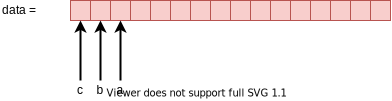
\includegraphics[height=0.4\textheight]{figures/pointeraliasing.png}
  \end{center}
\end{frame}

\begin{frame}[fragile]
  \frametitle{Solutions to pointer aliasing}
  \begin{enumerate}[itemsep=9pt]
  \item<1-> Some compilers can handle it on their own
    \begin{itemize}[itemsep=4pt]
    \item Multiple versions of the loop are generated
    \item Run-time check for aliasing
    \item Appropriate version is used
    \end{itemize}
  \item<2-> Tell the compiler with \texttt{-fno-alias}
  \item<3-> We can guarantee pointers will not alias
    \begin{itemize}[itemsep=4pt]
    \item \texttt{double * restrict} (in C99 or newer)
    \item \texttt{double * \_\_restrict\_\_} (in C++)
    \end{itemize}
  \end{enumerate}
\end{frame}





\begin{frame}[fragile]
  \frametitle{Compiler loop-specific \texttt{\#pragma} directives}

\begin{lstlisting}
#pragma <directive>\n
<for_loop>
\end{lstlisting}

  \vskip 8pt

  \structure{Ignore vector dependencies}
  \begin{itemize}[itemsep=5pt, topsep=6pt]
  \item \parbox{1.2cm}{\structure{\texttt{g++}}}:
    \parbox{6cm}{\texttt{\#pragma GCC ivdep}}
    \href{https://godbolt.org/z/49qd16PTP}{\faCog}
    \raisebox{1pt}{$\Rightarrow$}
    \href{https://godbolt.org/z/fGvsTqo43}{\faCog}

  \item \parbox{1.2cm}{\structure{\texttt{icpc}}}:
    \parbox{6cm}{\texttt{\#pragma ivdep}}
    \href{https://godbolt.org/z/WcP6conYc}{\faCog}
    \raisebox{1pt}{$\Rightarrow$}
    \href{https://godbolt.org/z/8fc68x4ad}{\faCog}/%
    \href{https://godbolt.org/z/bKh1qYd1d}{\faCog}
    (\texttt{GCC} ignored)
  \end{itemize}

  \vskip 8pt
  \structure{Force loop unrolling factor}
  \begin{itemize}[itemsep=5pt, topsep=6pt]
  \item \parbox{1.2cm}{\structure{\texttt{g++}}}:
    \parbox{9cm}{\texttt{\#pragma GCC unroll(<factor>)}}
    \href{https://godbolt.org/z/3s1a5sh9G}{\faCog}
    \raisebox{1pt}{$\Rightarrow$}
    \href{https://godbolt.org/z/WxWeb8bnf}{\faCog}

  \item \parbox{1.2cm}{\structure{\texttt{icpc}}}:
    \parbox{9cm}{\texttt{\#pragma unroll(<factor>)}}
    \href{https://godbolt.org/z/Pos7vWErT}{\faCog}
    \raisebox{1pt}{$\Rightarrow$}
    \href{https://godbolt.org/z/36eMKf3Y1}{\faCog}
  \end{itemize}

\end{frame}





\begin{frame}[fragile]
  \frametitle{OpenMP vectorisation \texttt{\#pragma} directives\hfill
    \href{https://www.openmp.org/spec-html/5.0/openmpsu42.html}
    {\large \faQuestionCircle}\;}
  \vspace{6pt}
\begin{lstlisting}
#pragma omp simd [<clause>[[,]<clause>]]...]\n
<for_loop>
\end{lstlisting}
  \vspace{6pt}
  For \structure{vertical} operations, \verb#<clause># can be
  \vspace{6pt}
  \begin{itemize}[wide=0pt,itemsep=6pt,topsep=6pt]
  \item \verb#safelen(<length>)#: unrolling factor safe to use.
  \item \verb#simdlen(<length>)#: number of SIMD lanes to use.
  % \item \verb#uniform(<var>)#: variable doesn't change value.
  \item \verb#linear(<list>[:<step>])#: step for variables in \verb#<list>#.
  \item \verb#if([simd :] <expr>)#: vectorise only if \verb#<expr># is true.
  \item \verb#collapse(<num>)#: collapse \verb#<num># levels of nested loops.
  \end{itemize}
\end{frame}





\begin{frame}[fragile]
  \frametitle{Reduction}
  For \structure{horizontal} operations, \verb#<clause># can be
  \vspace{11pt}
\begin{lstlisting}
reduction([<modifier>,]<identifier>:<list>)
\end{lstlisting}
  \vspace{11pt}
  where \verb#<identifier># can be
  \begin{itemize}[wide=0pt,itemsep=11pt,topsep=11pt]
  \item an arithmetic operation: \verb#+#, \verb#*#, \verb#-#,
    \verb#max#, \verb#min#
  \item a logical or bitwise operation: \verb#&#, \verb#&&#,
    \verb#|#, \verb#||#, \verb#^#
  \end{itemize}
  \vspace{5pt}
  and \verb#<list># is a list of variables. For \verb#<modifier>#s, see
  \href{https://www.openmp.org/spec-html/5.0/openmpsu107.html}{\faQuestionCircle}.

\end{frame}





\begin{frame}[fragile]
  \frametitle{Vectorised functions}
  {\small
\begin{lstlisting}
#pragma omp declare simd [<clause>[[,]<clause>]...]\n
[#pragma omp declare simd [<clause>[[,]<clause>]\n]
[...]
<function_definition_or_declaration>
\end{lstlisting}}

    \vskip 16pt

    \begin{itemize}[wide=0pt, itemsep=11pt, topsep=11pt]
    \item Generates multiple (vectorised) versions of the function.
    \item \structure{However}, compilers will often inline, then vectorise.
    \item Use \verb#-fno-inline# (\verb#g++#) or
      \verb#-qno-inline# (\verb#icpc#) to check.
    \end{itemize}

\end{frame}





  \begin{frame}[fragile]
  \frametitle{Some examples}
  \begin{itemize}[wide=0pt, itemsep=7pt, topsep=7pt]
  \item \parbox{10cm}{Ignoring vector dependencies}
    \href{https://godbolt.org/z/jTzGnvo78}{\faCog}
    \raisebox{1pt}{$\Rightarrow$}
    \href{https://godbolt.org/z/jbhjbqnxv}{\faCog}

  \item \parbox{10cm}{Safe forward dependencies}
    \href{https://godbolt.org/z/b8TTafEE1}{\faCog}
    \raisebox{1pt}{$\Rightarrow$}
    \href{https://godbolt.org/z/sebheva11}{\faCog}
    \raisebox{1pt}{$\Rightarrow$}
    \href{https://godbolt.org/z/Yq7jfq1xn}{\faCog}

  % \item \parbox{10cm}{}
  %   \href{}{\faCog}
  %   \raisebox{1pt}{$\Rightarrow$}
  %   \href{}{\faCog}

  % \item \parbox{10cm}{}
  %   \href{}{\faCog}
  %   \raisebox{1pt}{$\Rightarrow$}
  %   \href{}{\faCog}

  \item \parbox{10cm}{Reduction in inner product}
    \href{https://godbolt.org/z/sfYM7cedq}{\faCog}
    \raisebox{1pt}{$\Rightarrow$}
    \href{https://godbolt.org/z/eqrcTvWE9}{\faCog}

  \item \parbox{10cm}{Declare SIMD function}
    \href{https://godbolt.org/z/o55vPqY9z}{\faCog}
    \raisebox{1pt}{$\Rightarrow$}
    \href{https://godbolt.org/z/EKEnxYPxc}{\faCog}

  \end{itemize}

  \vskip 11pt
  \pause

  \structure{USEFUL REMINDERS}
  \begin{itemize}[wide=0pt, itemsep=7pt, topsep=7pt]
  \item Don't forget \verb#-fopenmp# (\verb#g++#) or
    \verb#-qopenmp# (\verb#icpc#)!
  \item  \verb#-fopt-info# (\verb#g++#) and
    \verb#-qopt-report# (\verb#icpc#) can help.
  \item \parbox{10cm}{Memory \structure{must be contiguous}}
    \href{https://godbolt.org/z/n6sEK79d3}{\faCog}
    \raisebox{1pt}{$\Rightarrow$}
    \href{https://godbolt.org/z/9hdKvo6ez}{\faCog}
  \end{itemize}

\end{frame}




\end{document}
%%% Local Variables:
%%% mode: latex
%%% TeX-master: t
%%% End: